\section{Redox-Reaktionen}

\subsubsection{Definition}
\begin{tabular}{l l}
	Oxidationsmittel \textbf{(OM)} & der Stoff, der Elektronen aufnimmt                  \\
	                               & und \textbf{reduziert} wird ($+e^-$)                       \\
	Reduktionsmittel \textbf{(RM)} & der Stoff, der die Elektronen abgibt                \\
	                               & und \textbf{oxidiert} wird ($-e^-$)                        \\
\end{tabular}

\subsubsection{Oxidationszahl}
$\rightarrow$ \textbf{F ist immer I, O fast immer -II, H fast immer +I} \newline
Die Oxidationszahl ist die Essenz der Redoxreaktion:
\begin{itemize}
	\item Um zu erkennen, wie viele Elektronen ein Stoff abgibt oder aufnimmt 
	\item es zeigt, welche Valenzelektronen bindungsfähig sind (Ladungen). 
	\item Elektronennegativere übernimmt die Elektronenladung \newline (z. B. C bei einer C H- Bindung, bei C-O nimmt O Ladung). 
\end{itemize}
\textbf{Wichtig:} die Gesamtladung muss, die Gleiche sein wie das Teilchen / Molekül angibt (zB. $\ce{F3P^0}$)\newline 
\begin{center}
	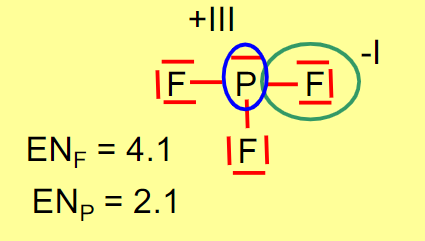
\includegraphics[height=1cm]{images/OZ.png}
\end{center}

\subsection{Redox Reaktionsgleichung - Ablauf}

\begin{enumerate}
	\item \textbf{Findet eine Reaktion überhaupt statt?} \\
	Man liest die Redoxreihe von \textbf{links nach rechts}. \\
	\textbf{oxidierte Form} reagiert mit \textbf{reduzierten Form}, die \textbf{unter ihr} in der Redoxreihe steht – das nennt man eine \textit{Bergab-Stellung}.
	\item \textbf{Edukte} kommen auf die \textbf{linke Seite}, \textbf{Produkte} auf die \textbf{rechte Seite} der Reaktionsgleichung.
	\item \textbf{Oxidationszahl} nachschauen und in römische Ziff. angeben	
	\item \textbf{Ausgleichen} der Reaktionsgleichung (Elektronen-, Massen- und Ladungsausgleich).
\end{enumerate}

\begin{tabular} {l l l l}
	Ox: & $\ce{Fe^0}$ & $\rightarrow$ & $\ce{Fe^{2+}} + 2e^-$ \\
	Red: & $\ce{Cl^{0}2}+ 2e^-$ & $\rightarrow$ & $\ce{2Cl^{-1}}$ \\
	\hline
	$\ce{Fe_{(s)} + Cl2_{(g)}} + 2e^-$& $\ce{<=>}$ & $\ce{Fe^{2+} + 2Cl^- + 2e^-}$ & $\hat{=} \ce{FeCl2_(s)}$ 
\end{tabular}
\subsection{Nernst-Gleichung - Redoxpotential}
Die Nernst-Gleichung ist eine Formel, um das Elektrodenpotential einer Halbzelle unter nicht-Standardbedingungen zu berechnen. \newline
$\boxed{E = E^0+ \frac{0.06V}{z}\cdot lg \frac{Ox}{Red}}$ \newline
$\rightarrow$ ox und red wird in $\frac{mol}{L} = M$ angegeben und in der Aufgabe gegeben \newline
Metalle = 1

\subsubsection{Anwendung}
 Spannung galvanische Zelle: $U = \ce{E^{Kathode}} - \ce{E^{Anode}} V$

Anode = Oxidation $\qquad$ Kathode = Reduktion